\section{Pre-Defined Kernels Templates in SmlCL}

Since the kernels generated using \texttt{mkKern1} and
\texttt{mkKern2}, always follow the same strict pattern where each
instance of the kernel assigns a value to its corresponding slot in
the output buffer, they have limited practical uses. For example, it
is not possible to create a kernel that sums all of the elements in an
array.

In order to allow users to perform some of the common functions on
collections of values, like map and reduce, we have extended SmlCL
with some convenience functions for common operations.

\subsection{Map}

\begin{lstlisting}[language=ML,mathescape,caption=Signature for \texttt{map}]
val map : machine $\to$ ($\alpha$ expr $\to$ $\beta$ expr) $\to$ $\alpha$ T $\to$ $\beta$ T $\to$ ($\alpha$, $\beta$)kern1
\end{lstlisting}

The \texttt{map} function is used to create a kernel that maps a
function onto a buffer in parallel, with the result ending up in a new
buffer. For example, the expression
\begin{lstlisting}[language=ML,label=mapkern,caption=Sample call to \texttt{map}]
  map m (fn x => Div (Mul x x) (RealC 1.5)) Int Int
\end{lstlisting}
will yield the following kernel
\begin{lstlisting}[language=C,label=vectoradd,caption=Resulting kernel
  from the call in listing \ref{mapkern}.]
  #pragma OPENCL EXTENSION cl_khr_fp64 : enable
  
  __kernel void map(__global double* buf1,
                    __global double* bufr) {
    int iGID = get_global_id(0);
    bufr[iGID] = ((buf1[iGID] * buf1[iGID]) / 1.5);
  }
\end{lstlisting}

As such, it is a rather straightforward implementation, and could have
been approximated by the user of SmlCL like this:

\begin{lstlisting}[language=ML,caption=Approximation of \texttt{map}
    function.]
  mkKern1 m "map" (fn x => Add (x This) (x This)) Int Int
\end{lstlisting}

Except that we then have to directly specicify which index
(\texttt{This}) into the buffer we are operating on.

Since this is a rather straightforward function, it doesn't offer a
lot of room for fine-tuning, which unfortunately also means that it is
not all that fast compared to traditional sequential code.

\begin{table}
  \center
  \label{maptable}
  \begin{tabular}{l|l}
    CPU  & GPU  \\ \hline
    5452 ms & 4500 ms \\ \hline
    5452 ms & 4496 ms \\ \hline
    6048 ms & 4780 ms \\ \hline
  \end{tabular}
  \caption{Measurements of execution time for a simple operation on
    each element of an array.}
\end{table}

Table \ref{maptable} shows three measurements of how long it took (in
milliseconds) to run the program in appendix \ref{app:map}, using the
GPU and the CPU respectively. The code performs a simple mapping like
the one in listing \ref{mapkern} a hundred times on a randomly
generated array of reals.

As we can see, the GPU code actually performs slower than the CPU
code. This is due to the fact that we have to generate the array of
random numbers on the host-side and transfer it to the GPU device
before we can even start working on it. Data-transfer is very slow
compared to data-processing, and acts as a bottle-neck for this
test. In order to achieve better performance, the GPU kernel has to be
more computationally expensive, so that the time of computation
greatly outweighs the time of transfer. A better approach would be to
generate the random numbers on the GPU device itself. Unfortunately,
the OpenCL run time does not support traditional C-like random number
generation using \texttt{rand()}. Instead, we can chose a uniform
distribution of numbers between $0$ and $1.0$ and let the kernel
generate those. This approach will be demonstrated later in chapter
\ref{sec:pi}.

\subsection{Reduce}

The \texttt{red} function is the parallel equivalent of the
traditional \texttt{reduce} function. It takes a function from $\alpha
* \beta$ to $\beta$, and iteratively applies that function to elements
of the input buffer, accumulating the results in the second parameter.

\begin{lstlisting}[language=ML,mathescape,caption=Signature for \texttt{red}.]
  val red : machine $\to$ ($\alpha$ expr * $\beta$ expr $\to$ $\beta$ expr) $\to$ $\beta$ expr $\to$ $\alpha$ T $\to$ $\beta$ T $\to$ ($\alpha$, $\beta$)kern1
\end{lstlisting}


For example \texttt{red m (Add x x) (IntC 0) b Int} where \texttt{b}
is a buffer of type \texttt{int buf}, would return the sum of all the
elements in the buffer. Note that this function, unlike map, does not
return a kernel, but immediately returns the result.

Reductions on the GPU can be done in a number of ways. The most simple
is to have a single thread iteratively go through the entire array and
calculate the reduction, but then we are just doing the reduction
sequentially and might as well do it on the CPU. Instead, we can
choose to take advantage of the associative and commutative properties
of many common reduction operations. For example, if we simply want to
calculate the sum of all elements in an array, or find the highest or
lowest value, we do not care in which order the elements are
processed. One way to take advantage of this, is to have each kernel
separately compute intermediate reductions for part of the array,
followed by a single reduction of the intermediate results. Our
reduce-kernel follows this approach, by having each kernel calculate
the reduction of part of the input array and store it in the output
buffer at the position corresponding to their global id, waiting for
all kernels to sync up, and then having the first kernel (with global
ID 0) sum up the intermediate results into the first location in the
output buffer. 

Because of the way the reduction is computed, we felt that it would be
easiest to let \texttt{red} automatically extract the result from the
output buffer, which is why it cannot simply return a kernel.

\subsection{Approximating $\pi$.}
\label{sec:pi}

We saw above that mapping a relatively simple function onto an array
using SmlCL did not yield much, if any, improvement in performance. We
are now going to focus on something a little more computationally
demanding: approximating $\pi$.

Suppose you have a circle of radius $1$ inside a square of width
$2$. The area of the circle $a_c$ is $\pi r^2 = \pi$, the area of the
square $a_s$ is $2*2=4$, and the ratio $a_c \over a_s$ is $\pi \over
4$. That means, that if we arbitrarily sample points within the
square, the chance that it is within the circle as well is $\pi \over
4$. We can even split the square up into 4 parts, representing the
quadrants in a regular graph, and since each quadrant is simply an
mirrored image of the other quadrants, we can simply sample points
within one of the quadrants estimate $\pi$. Simply put, if we randomly
select $n$ numbers $x_1, \ldots, x_n$ and $y_1, \ldots, y_n$, between
$0$ and $1$, the amount of points $(x_i, y_i)$ for which $x_i^2 +
y_i^2 \leq 1$ is approximately $\pi n \over 4$. This is called the
Monte Carlo method for $\pi$.

\begin{figure}[h]
  \center
  \caption{Sampling of points in a circle. Source: \url{http://math.fullerton.edu/mathews/n2003/montecarlopimod.html}}
  \label{fig:pi1}
  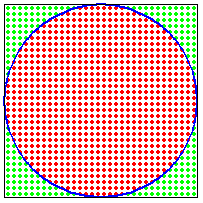
\includegraphics[scale=0.5]{figures/pi1.png}
\end{figure}

Using this knowledge, we can use the \texttt{map} and \texttt{red}
functions to estimate $\pi$. Table \ref{table:pi} shows the result of
computing $\pi$ using this method. Each simulation runs 100 times and
uses 1000000 randomly generated numbers. The source code is listed in
appendix \ref{app:pi}. 

\begin{table}
  \center
  \label{table:pi}
  \begin{tabular}{l|l}
    CPU & GPU \\ \hline
    11964 ms & 11500 ms \\ \hline
    10332 ms & 11308 ms \\ \hline
    9132 ms & 10864 ms \\ \hline
  \end{tabular}
  \caption{Estimating $\pi$ using the Monte Carlo method. The code can
  be seen in appendix \ref{app:pi}.}
\end{table}

The parallel program performs about as fast as the sequential
one. Again, this must be attributed to the high cost of transferring
data to the device, compared to the relative simple computation
taking place.

To properly take advantage of the capabilities of the GPU, it is clear
that we must minimize data transfer, and perform as much computation
on the GPU as possible. One way we could get better performance in our
benchmark above, would be to have the GPU generate the random numbers
itself. Unfortunately, the OpenCL runtime does not provide standard
\texttt{rand()} type functions. 

If we, instead of relying on random numbers, simply generate a list of
numbers from $0$ to $1$, like $0.0, 0.0, 0.1, \ldots, 1.0$, we still
get the same distribution of points inside the circle, but without the
random element. This allows us to let the kernels calculate their
points individually, and thus we avoid having to transfer a large
buffer of numbers to the device before we can start computing.

\begin{table}
  \center
  \label{table:altpi}
  \begin{tabular}{l|l}
    CPU & GPU \\ \hline
    78556 ms & 1100 ms \\ \hline
    78436 ms & 1088 ms \\ \hline
    78168 ms & 1096 ms \\ \hline
  \end{tabular}
  \caption{Estimating $\pi$ using evenly distributed
    numbers from $0$ to $1$.}
\end{table}

Unfortunately, the current expression generator functions in SmlCL are
not powerful enough to express such a kernel. Thankfully, we can use
PrimCL instead and supply it with a manually coded kernel. Table
\ref{table:altpi} shows the results of running the code in appendix
\ref{app:altpi}, showing a significant performance boost from using
the GPU compared to the CPU. This indicates that, in order to take
full advantage of the parallel architecture of the GPU, we have to
extend the SmlCLs expression generator capabilities to allow more
advanced constructions such as loops.
